
%(BEGIN_QUESTION)
% Copyright 2005, Tony R. Kuphaldt, released under the Creative Commons Attribution License (v 1.0)
% This means you may do almost anything with this work of mine, so long as you give me proper credit

The starter and overload heater assembly for an industrial electric motor is often located quite a distance from the motor itself, inside a room referred to as a {\it motor control center}, or MCC:

$$\includegraphics[width=15.5cm]{i02312x01.eps}$$

Since it is impossible for a technician to be in two places at once, it is often necessary to perform diagnostic checks on a malfunctioning electric motor from the MCC where the technician has access to all the control circuitry.

One such diagnostic check is line current, to detect the presence of an open motor winding.  If a three-phase motor winding fails open, or if one of the three-phase power conductors fails open along the way to the motor, the motor will not run as it should.  This is called {\it single-phasing}.  A good way to check for this condition is to use a clamp-on (inductive) ammeter to check line current on all three lines while the starter is energized.  This may be done at any location where there is physical access to the motor power conductors.

\goodbreak

Suppose, though, you are working on a job site where single-phasing is suspected and you do not have a clamp-on ammeter with you.  All you have is a DMM (digital multimeter), which does not have the ability to safely measure the motor's current.  You are about to head back to the shop to get a clamp-on ammeter when a more experienced technician suggests an alternate test.  He takes your DMM, sets it to the AC {\it millivolt} range, then connects the test probes to either side of each overload heater element, one heater at a time like this:

$$\includegraphics[width=15.5cm]{i02312x02.eps}$$

Across each overload heater element he measures about 20 mV AC with the starter engaged.  From this he determines that the motor is {\it not} single-phasing, but is drawing approximately equal current on all three phases.

Explain how this diagnostic check works, and why this determination can be made.  Also describe what limitations this diagnostic procedure has, and how a clamp-on ammeter really is the best way to measure motor line current.

\underbar{file i02312}
%(END_QUESTION)





%(BEGIN_ANSWER)

Each overload heater element possesses a small amount of electrical resistance, which is the key to this diagnostic procedure.  Of course, the measurement obtained is strictly qualitative, not quantitative as a clamp-on ammeter would give.

\vskip 10pt

Follow-up question \#1: what sort of result might occur with this diagnostic check if the motor were indeed single-phasing due to one of the overload heaters failing open?

\vskip 10pt

Follow-up question \#2: what other causes could there be for a three-phase motor ``single-phasing'' other than a motor winding failed open?

%(END_ANSWER)





%(BEGIN_NOTES)

I have used this diagnostic check more than once to troubleshooting a single-phasing electric motor.  It is amazing what sorts of diagnostic checks you can do with a high-quality DMM and a sound understanding of electrical theory!

%INDEX% Electronics review: AC motor control circuit

%(END_NOTES)


